\documentclass[11pt]{article}

\usepackage[margin=1in]{geometry}
\usepackage[T1]{fontenc}
\usepackage[utf8]{inputenc}
\usepackage{lmodern}
\usepackage{microtype}
\usepackage{amsmath,amssymb,amsthm}
\usepackage{booktabs}
\usepackage{graphicx}
\usepackage[numbers]{natbib}
\usepackage[hidelinks]{hyperref}

\newtheorem{proposition}{Proposition}
\newtheorem{lemma}{Lemma}
\newtheorem{corollary}{Corollary}
\theoremstyle{definition}
\newtheorem{definition}{Definition}

\newcommand{\Ct}{C_t}
\newcommand{\E}{\mathbb{E}}
\newcommand{\R}{\mathbb{R}}
\newcommand{\clip}{\operatorname{clip}}

\title{\textbf{Working draft:} Deliberate Competence Evolution in Heterogeneous Learning Systems}
\author{Anonymous working draft}
\date{\today}

\begin{document}
\maketitle

\begin{abstract}
This working draft frames Heterogeneous Learning Systems (HLS) as evolving organizations of competence. It distinguishes work allocation from knowledge and learning allocation, describes a provisional collaborative architecture, and records a scaffold for a theory of competence orchestration. The draft preserves a small set of two-learner/two-task analytical results and numerical consistency checks as preliminary, model-scoped evidence. General integration theory and realistic experimental validation remain open. The draft makes no novelty claim and does not establish RQ0, a general HLS result, or a coupling advantage over a fully informed modular controller.
\end{abstract}

\section{Introduction}

Modern AI systems can combine models, agents, or other learners with different quality, cost, latency, competence, and learning profiles. Their immediate operational question is familiar: which member should handle the current task? If members can learn, however, this view is incomplete. Operation can generate experience; capable interventions can generate potentially reusable knowledge; and learning can change future competence.

The programme-level motivation is a feedback loop:
\begin{equation}
\begin{gathered}
\text{heterogeneous learners} \rightarrow \text{operation and routing} \rightarrow \text{experience}\\
\rightarrow \text{learning or transfer} \rightarrow \text{competence redistribution}\\
\rightarrow \text{future operation}.
\end{gathered}
\label{eq:cycle}
\end{equation}
The system consequently faces two linked allocation problems: work allocation and knowledge or learning allocation. Together they determine a future organization of competence, rather than only use a current one. We use a provisional hierarchical and collaborative language of inexpensive learners and capable teachers: teachers can provide service and potentially useful knowledge, while learners can absorb demand and adapt. These are functional roles, not fixed types.

Environmental dynamics make the distinction especially relevant. A persistent change in demand, costs, latency requirements, resources, constraints, or required competences can make a previously useful organization less suitable. Whether an HLS can deliberately reorganize its competences to create long-term value is a hypothesis, not an established response to change.

The repository-level research question is:
\begin{quote}
Can the deliberate evolution of competence allocation in a heterogeneous learning system improve its long-term performance compared with independently optimizing task allocation and knowledge transfer?
\end{quote}
This draft does not replace RQ0.

Closed-loop routing and learning already have direct operational precedent. For example, RouteNLP uses routing failures to select targeted distillation data and subsequently recalibrates routing \citep{guo2026routenlp}. Cross-domain models also integrate work assignment, competence dynamics, and training \citep{borgonjon2024dynamic}. These precedents constrain component claims; they do not by themselves settle the programme-level question.

The purpose of the paper is conservative. It documents a provisional HLS architecture, an integration-theory scaffold, and preliminary minimal analytical results with numerical consistency checks. The architecture and general theory are still being developed; general experiments do not yet exist. The results therefore do not establish novelty, general HLS superiority, realistic empirical validation, or the candidate coupling proposition P4.

\section{Problem formulation and design objectives}

An HLS is not only a portfolio of heterogeneous components to be exploited at the current time. It is an evolving organization of usable competences. Let the provisional competence portfolio be $\Ct=[c_{iz}(t)]$, where $c_{iz}(t)$ denotes effective competence of member $i$ for task region $z$. This is conceptual notation: competence need not be directly observable, and it is not assumed to be identical to accuracy or a sufficient state representation.

At time $t$, the environment $E_t$ includes the task demand and may also affect costs, latency requirements, resource availability, operational constraints, and required competences. It may be stationary or change over time. The design objective is not an artificial objective of maximizing diversity or every $c_{iz}$ independently. It is to understand when the organization of competences has functional value for long-horizon system operation.

Two linked allocation problems follow:
\begin{equation}
\text{who should solve now?}\qquad \neq \qquad \text{who should learn?}
\label{eq:two-allocations}
\end{equation}
The first selects a current division of labour. The second decides whether knowledge generated by operation or by a capable intervention should be retained, transferred, or used to transform one or more members. The member that fails, serves a task, or produces knowledge need not be the member that should learn.

The repository-level research question remains:
\begin{quote}
Can the deliberate evolution of competence allocation in a heterogeneous learning system improve its long-term performance compared with independently optimizing task allocation and knowledge transfer?
\end{quote}
It is a scientific hypothesis, not a result of this paper. The long-horizon comparison must be conditioned on a specified environment, horizon, information set, resources, and strong alternatives.

The design objectives of this draft are therefore modest: make the architecture and its candidate decisions explicit; identify importable foundations and their structural limits; preserve preliminary minimal-model evidence; and state how a future validation programme could test the general question without presuming a positive outcome.

\section{Cross-domain foundations and related work}

This section is organized by function within the architecture, not by ownership claims. The methodological rule is to import mechanisms and mathematical tools without importing or replacing the HLS research problem.

\paragraph{Heterogeneous routing and hierarchical inference.} Dynamic routing systems such as RouteNLP and MixLLM provide direct precedents for selecting among heterogeneous models, including targeted distillation after routing failures in RouteNLP \citep{guo2026routenlp,wang2025mixllm}. They motivate strong routing baselines. They do not by themselves define a general competence organization or long-horizon portfolio objective.

\paragraph{Learning, Machine Teaching, and knowledge transfer.} Iterative Machine Teaching studies learner-aware sequential intervention and incomplete learner information \citep{liu2017iterative,liu2018blackbox}. Iterative Classroom Teaching additionally treats heterogeneous learner states and rates, shared examples, grouping, orchestration cost, and a fixed exogenous target $w^*$ \citep{yeo2019iterativeclassroom}. These provide mechanisms for teaching heterogeneous learners, not a target competence allocation chosen from future collective operation. Selective transfer in continual learning further motivates non-scalar transition effects \citep{lee2021sharing}.

\paragraph{Competence development and workforce skill allocation.} Borgonjon and Maenhout jointly model staffing, task assignment, learning-by-doing, forgetting, explicit training, shadow training, dynamic skill mix, and skill-dependent future operational efficiency \citep{borgonjon2024dynamic}. This is a serious structural precedent for dynamic operation and competence development. Its normative objective is workforce staffing cost under a prescribed task and scheduling environment; it does not alone establish RQ0 or a general artificial-learning portfolio objective. The repository's targeted audit records the exact bounded comparison.

\paragraph{Distributed organizational knowledge and specialization.} Transactive-memory systems provide a conceptual account of who knows what, complementary expertise, coordination, path dependence, and knowledge reconfiguration \citep{argote2012transactive}. They show why collective capability need not reduce to isolated expertise, but they do not formulate a normative dynamic optimization that selects artificial learners' competence acquisitions by downstream operational utility.

\paragraph{Portfolio, resource allocation, and dynamic adaptation.} Decision-aware active learning, graph-triggered allocation, and decision-focused optimization separate immediate prediction or reward from later decision value \citep{bickfordsmith2023prediction,filstroff2024targeted,genalti2024graph,elmachtoub2021smart,wang2023scalable}. The Gutjahr competence-development line, identified in the repository's cross-domain audit, is also an apparatus source for competence states, nonlinear efficiency mappings, trajectories, and strategic development; exact paper-bibliography entries remain a documented TODO rather than invented citations.

The integration perspective is therefore not a claim that known components become novel by juxtaposition. It asks how their roles, assumptions, endogenous quantities, and comparison classes translate into an HLS architecture. A structural reduction to strong prior models is required before claiming any residual.

\section{Provisional collaborative HLS architecture}

The architecture is a functional decomposition, not a proposed centralized algorithm or a claim that all HLS instances must use the same roles.

\paragraph{A1: Distributed heterogeneous competence.} The population contains actors with different competences, costs, latencies, specializations, and learning capacities. Heterogeneity is relevant only insofar as it has functional value for the system; the architecture imposes no separate diversity-maximization objective.

\paragraph{A2: Hierarchical and collaborative division of labour.} We provisionally call some functional roles \emph{students/learners} and \emph{teachers}. Students are often faster or cheaper and may be functionally specialized, so they should absorb substantial demand when appropriate. Teachers are often more capable but more costly or slower; they can solve tasks that students should not solve and can generate knowledge useful for later learning. These are roles, not rigid ontological types: an architecture may contain multiple teachers, multiple students, and horizontal heterogeneity among both.

\paragraph{A3: Selective learning and knowledge allocation.} Work allocation and learning allocation are distinct as in Equation~\eqref{eq:two-allocations}. A teacher intervention can supply current service, diagnostic information, and reusable teaching material simultaneously. The architecture must decide which knowledge to retain, which competence to develop, and which recipient should receive it.

\paragraph{A4: Competence-portfolio evolution.} The dynamic object is the trajectory $C_t\rightarrow C_{t+1}\rightarrow\cdots$, rather than an instruction to improve every member. \emph{Specialize}, \emph{broaden}, \emph{replicate}, and \emph{rebalance} are possible transformation families whose value depends on the environment and constraints; they are not independent results.

\paragraph{A5: System-level orchestration.} A conceptual orchestration function integrates the architecture. It asks who should act now, when a teacher should intervene, what useful knowledge has been generated, who should learn it, and what competence organization should be built for later operation. No particular centralized implementation is assumed.

\begin{figure}[t]
\centering
\fbox{\begin{minipage}{0.91\linewidth}
\centering\small
\textbf{Environment $E_t$ and demand} $\downarrow$ \quad \textbf{System-level orchestration (A5)}\\[2pt]
\textbf{Work flow:} operational allocation $\longrightarrow$ students / teachers $\longrightarrow$ service and operational experience\\[2pt]
\textbf{Knowledge flow:} experience or teacher output $\longrightarrow$ knowledge selection / learning allocation $\longrightarrow C_{t+1}$\\[2pt]
$C_{t+1}$ feeds future operational allocation. Teachers can solve and provide potential knowledge; students can solve and learn. The two flows are distinct but coupled.
\end{minipage}}
\caption{Conceptual architecture of the working HLS model. This schematic is a design scaffold, not a finalized architecture or empirical result.}
\label{fig:hls-architecture}
\end{figure}

The resulting coupled cycle is
\begin{equation}
\begin{aligned}
C_t &\rightarrow \text{work allocation} \rightarrow \text{experience / teacher intervention}\\
&\rightarrow \text{knowledge allocation} \rightarrow \text{learning} \rightarrow C_{t+1}\\
&\rightarrow \text{future work allocation}.
\end{aligned}
\label{eq:hls-cycle}
\end{equation}
Environmental dynamics are not a sixth architectural pillar. They are a condition under which the same architecture can be studied: $E_{t+1}=E_t$ in a stationary regime, or $E_{t+1}\neq E_t$ when relevant environmental elements change.

\section{Theory of competence orchestration: integrated investment scaffold}

This section gives one \textbf{CANDIDATE / WORKING-HYPOTHESIS} value model for the A1--A5 architecture. It is not a final integration theory, an algorithm, or a general HLS result. R1--R3 are three resolutions of one competence-investment decision: whether to invest, where to place an intervention, and what portfolio organization to construct.

Let $C_\tau^a$ denote the counterfactual competence trajectory after intervention $a$, and $C_\tau^0$ the no-investment trajectory. Let $U^*(C,E)$ be the best feasible operational utility available to the portfolio in environment $E$. Define competence-investment value (CIV) by
\begin{equation}
\mathrm{CIV}_t(a)=-K_t(a)+\E\!\left[\sum_{\tau=t+1}^{H}\gamma^{\tau-t}\left(U^*(C_\tau^a,E_\tau)-U^*(C_\tau^0,E_\tau)\right)\right].
\label{eq:civ-general}
\end{equation}
The expectation is conditional on information at $t$. Cost $K_t(a)$ includes the intervention resources and opportunity costs assigned to $a$. The no-investment action has $\mathrm{CIV}_t(0)=0$ by definition. CIV thus relates A3 learning allocation and A4 portfolio evolution to A2's feasible future division of labour; A5 may conceptually compare actions without assuming a particular centralized implementation.

\subsection{R1: whether to invest}

For a set $\mathcal A_I$ of candidate investments, invest rather than do nothing iff
\begin{equation}
\max_{a\in\mathcal A_I}\mathrm{CIV}_t(a)>0,
\label{eq:civ-invest}
\end{equation}
with boundary $\max_{a\in\mathcal A_I}\mathrm{CIV}_t(a)=0$. This is \textbf{DERIVED-IN-MODEL}: it follows from the stated counterfactual comparison, not from a claim that CIV is observable or optimal in real systems.

\subsection{A minimal CIV specialization}

For analysis, consider two students, one teacher, two task regions, and finite environment-dependent capacities. Let $R(C,E)$ be the feasible operational allocations and
\begin{equation}
U^*(C,E)=\max_{r\in R(C,E)}U(C,E,r).
\label{eq:civ-operational-value}
\end{equation}
Let $E_t$ be Markov with persistence $\rho$, for example $P_\rho=\rho I+(1-\rho)Q$. An action $a$ has cost $K_a$, success probability $\eta_a$, and learning delay $\delta_a$. Conditional on success, it applies a specified transformation $T_a$ after the delay; conditional on failure it leaves the comparison portfolio unchanged. With success conditionally independent of the environment path, define
\begin{equation}
m_a(E,C)=U^*(T_a(C),E)-U^*(C,E),
\label{eq:marginal-operational-value}
\end{equation}
and obtain
\begin{equation}
\mathrm{CIV}_t(a)=-K_a+\eta_a\E\!\left[\sum_{\tau=t+\delta_a}^{H}\gamma^{\tau-t}m_a(E_\tau,C_\tau^0)\right].
\label{eq:civ-specialized}
\end{equation}
The factorization by $\eta_a$ is specific to this binary-success specialization. Marginal value can depend on future demand, exposure, capacity and availability scarcity, teacher substitution cost, learning speed, and delay.

\subsection{R2: where to invest}

Let $g_a$ be an action's local recipient competence gain and define $L_t(a)=\E[\sum_{\tau=t+\delta_a}^{H}\gamma^{\tau-t}m_a(E_\tau,C_\tau^0)]$. A larger local gain need not yield larger CIV. For two actions, a reversal occurs when
\begin{equation}
g_a>g_b\quad\text{and}\quad \eta_aL_t(a)-\eta_bL_t(b)<K_a-K_b.
\label{eq:civ-reversal}
\end{equation}
For example, a large gain in a region already covered by an available specialist with slack capacity can have $L_t(a)=0$, while a smaller gain can relieve a binding capacity constraint or expensive teacher allocation. Hence such reversals exist under the specialization. This is \textbf{DERIVED-IN-MODEL}; it does not show their prevalence or supply an estimator of CIV.

\subsection{R3: organization through competing transformations}

Let $\mathcal A=\{S,R,B,0\}$ denote SPECIALIZE, REPLICATE, REBALANCE, and DO-NOTHING. These are competing transformations of one portfolio, not distinct models. For any two investments $a,b$, the pairwise boundary is
\begin{equation}
\mathrm{CIV}_t(a)=\mathrm{CIV}_t(b)
\quad\Longleftrightarrow\quad
\eta_aL_t(a)-\eta_bL_t(b)=K_a-K_b.
\label{eq:civ-boundary}
\end{equation}
Thus the $S/R$, $R/B$, and $S/B$ boundaries are obtained by substituting the corresponding actions into Equation~\eqref{eq:civ-boundary}; the investment/DO-NOTHING boundary is Equation~\eqref{eq:civ-invest}. These are \textbf{DERIVED-IN-MODEL} indifference identities, not empirical regime maps or general preferences for any transformation family.
Explicitly,
\begin{align}
\mathrm{CIV}_t(S)=\mathrm{CIV}_t(R)
&\Longleftrightarrow \eta_S L_t(S)-\eta_R L_t(R)=K_S-K_R, \\
\mathrm{CIV}_t(R)=\mathrm{CIV}_t(B)
&\Longleftrightarrow \eta_R L_t(R)-\eta_B L_t(B)=K_R-K_B, \\
\mathrm{CIV}_t(S)=\mathrm{CIV}_t(B)
&\Longleftrightarrow \eta_S L_t(S)-\eta_B L_t(B)=K_S-K_B.
\label{eq:civ-pairwise-boundaries}
\end{align}

\subsection{Null result and candidate buffering behaviour}

Environmental volatility alone does not imply replication. If existing specialists have adequate capacity and availability in every reachable environment, replication changes neither feasibility nor $U^*$; then $m_R(E,C)=0$, $L_t(R)=0$, and $\mathrm{CIV}_t(R)=-K_R\leq0$, even when $\rho$ is low. The operative determinants are their interaction: future demand, portfolio exposure, capacity and availability scarcity, teacher cost, learning cost and speed, adaptation delay, and environment persistence.

Teacher buffering is not an axiom. It is a \textbf{CANDIDATE / NOT ESTABLISHED} conditional behaviour: an environmental change can raise teacher load; teacher service can generate usable knowledge or experience; a positive-CIV intervention can reorganize the portfolio; and a later student allocation can reduce teacher load. Any link can fail, and neither this pattern nor CIV establishes novelty, general buffering value, superiority over strong modular control, RQ0, or P4.

The model imports apparatus from workforce learning/training, Machine Teaching, transactive memory, comparative advantage, portfolio, and control traditions. Borgonjon and Maenhout already integrate assignment, learning, training, forgetting, and future efficiency; Yeo et al. address heterogeneous learner-aware teaching toward an exogenous target; and Argote and Ren motivate configuration-dependent distributed expertise. CIV does not re-demonstrate these precedents or CR0--CR4; it provides a common candidate language for future structural reductions.

\section{Minimal analytical results / preliminary theory}

The following two-learner/two-task laboratory is retained because it makes selected null cases and interactions explicit. It is preliminary theory, not the narrative centre of the paper or a general HLS model. All propositions are scoped to their stated assumptions.

\section{A minimal two-learner/two-task model}

The following model is intentionally narrow. Learners $A,B$ and task regions $1,2$ have effective operational qualities
\begin{equation}
q_{iz}=c_{iz}-\lambda k_{iz}.
\label{eq:quality}
\end{equation}
Each learner has unit operational capacity, giving two divisions of labour:
\begin{equation}
D=(A\!\rightarrow\!1,B\!\rightarrow\!2),\qquad
X=(A\!\rightarrow\!2,B\!\rightarrow\!1).
\label{eq:divisions}
\end{equation}
Their values and difference are
\begin{equation}
R_D=q_{A1}+q_{B2},\quad R_X=q_{A2}+q_{B1},\quad
\Delta(C)=R_D-R_X.
\label{eq:division-values}
\end{equation}

\subsection{Assumptions and separability null case}

The model assumes two tasks, two learners, deterministic assignments, and no queues, abstention, mixed routing, transfer, interference, demand uncertainty, or shared training budget unless a later subsection explicitly introduces a coupling. It should not be read as a realistic HLS architecture.

Before adding capacity coupling, consider task-separable rewards and transitions:
\begin{equation}
R(C,a)=R_1(C_1,a_1)+R_2(C_2,a_2),\qquad
P(C'\mid C,a)=P_1(C'_1\mid C_1,a_1)P_2(C'_2\mid C_2,a_2).
\label{eq:separable}
\end{equation}
When no shared constraint or information couples the tasks, the Bellman maximisation factors. This null case is essential: a joint state notation alone does not create a joint competence-evolution problem.

\section{Theoretical results within the minimal model}

\subsection{CR0: separability}
\begin{proposition}[Separability null case]
Under Equation~\eqref{eq:separable}, additive rewards, and no shared constraints, the two-task dynamic decision problem decomposes into independent per-task problems.
\end{proposition}
\begin{proof}
Substitution of Equation~\eqref{eq:separable} into the Bellman recursion makes both the expectation and maximisation additive. Each action component can therefore be selected by the corresponding per-task maximisation.
\end{proof}
This is an \textbf{ESTABLISHED-IN-MODEL} null result. It ceases to apply when learner capacity, budget, data, teacher choice, interference, or a portfolio objective couples tasks.

\subsection{CR1: finite threshold and complementary investments}
Assume $Delta_0>0$, so $D$ is initially preferred. Improve $A2$ by $x\geq0$ and $B1$ by $y\geq0$, holding diagonal competences fixed. Then
\begin{equation}
\Delta'=\Delta_0-x-y,
\qquad
G(x,y)=[x+y-\Delta_0]_+.
\label{eq:complementarity}
\end{equation}
\begin{proposition}[Finite competence threshold]
Under the assumptions of Equation~\eqref{eq:complementarity}, two individually insufficient off-diagonal investments can jointly make $X$ preferable: if $x\leq\Delta_0$, $y\leq\Delta_0$, and $x+y>\Delta_0$, then $G(x,0)=G(0,y)=0$ while $G(x,y)>0$.
\end{proposition}
\begin{proof}
The investments add $x+y$ to $R_X$ and leave $R_D$ fixed. The conclusion follows directly from the positive-part expression in Equation~\eqref{eq:complementarity}.
\end{proof}
This is \textbf{ESTABLISHED-IN-MODEL}; it does not include learning cost, uncertain gain, or side effects.

\subsection{CR2: local specialization instability}
For the symmetric learning-by-doing case, let
\begin{equation}
r_D=\sigma(\beta\Delta),\qquad r_X=1-r_D,
\label{eq:router}
\end{equation}
and order the state as $(c_{A1},c_{B2},c_{A2},c_{B1})$. The dynamics are
\begin{align}
\dot c_{A1}&=\eta r_D(1-c_{A1})-\delta c_{A1}, &
\dot c_{B2}&=\eta r_D(1-c_{B2})-\delta c_{B2}, \nonumber\\
\dot c_{A2}&=\eta(1-r_D)(1-c_{A2})-\delta c_{A2}, &
\dot c_{B1}&=\eta(1-r_D)(1-c_{B1})-\delta c_{B1}.
\label{eq:lbd}
\end{align}
For positive $\eta,\delta$, the symmetric equilibrium is $c^*=\eta/(\eta+2\delta)$.

\begin{proposition}[Local assignment-asymmetry threshold]
At the symmetric equilibrium of Equation~\eqref{eq:lbd}, the assignment-asymmetry eigenvalue is
\begin{equation}
\lambda_{\mathrm{asym}}=-\frac{\eta+2\delta}{2}+\frac{2\eta\delta\beta}{\eta+2\delta}.
\label{eq:lambda-asym}
\end{equation}
It is zero at
\begin{equation}
\beta_c^{(2\times2)}=\frac{(\eta+2\delta)^2}{4\delta\eta}.
\label{eq:beta-critical}
\end{equation}
\end{proposition}
\begin{proof}
At $c^*$, define $s=(1,1,-1,-1)^T$, $L=(\eta+2\delta)/2$, and $\alpha=\eta\beta\delta/[2(\eta+2\delta)]$. The Jacobian is $J=-LI+\alpha ss^T$. Since $s^Ts=4$, it has three eigenvalues $-L$ and the eigenvalue in Equation~\eqref{eq:lambda-asym}; solving for zero gives Equation~\eqref{eq:beta-critical}.
\end{proof}
This is \textbf{ESTABLISHED-IN-MODEL} as a local stability result. It is not a global bifurcation theorem or a general claim that HLS should specialize.

\subsection{CR3 and CR4: rebalancing with two actuators}
Let $d_0>0$ be a scalar operational gap to a new division. Direct learning closes $x$ at cost $K_L(x)=ax$. If formative routing closes gap at $\dot d=-v$ and incurs instantaneous regret $d$, pure routing takes $\tau_R=d_0/v$ and has regret $K_R=d_0^2/(2v)$. With future advantage rate $g>0$,
\begin{equation}
H_R^*=\frac{d_0}{v}+\frac{d_0^2}{2vg},\qquad H_T^*=\frac{ad_0}{g}.
\label{eq:pure-rebalancing}
\end{equation}
If routing covers $y$ and training covers $x=d_0-y$, the effective cost is
\begin{equation}
Q(y)=a(d_0-y)+\frac{y^2}{2v}+\frac{gy}{v},\qquad 0\leq y\leq d_0.
\label{eq:q-y}
\end{equation}
\begin{proposition}[Two-actuator rebalancing]
For $v,g>0$, Equation~\eqref{eq:q-y} is strictly convex and has solution
\begin{equation}
y^*=\clip(av-g,0,d_0),\qquad x^*=d_0-y^*.
\label{eq:rebalancing-solution}
\end{equation}
Thus TRAIN applies when $av\leq g$, MIXED when $g<av<g+d_0$, and ROUTE when $av\geq g+d_0$. In the interior,
\begin{equation}
Q_M=ad_0-\frac{(av-g)^2}{2v},\qquad H^*=Q^*/g.
\label{eq:mixed-cost}
\end{equation}
\end{proposition}
\begin{proof}
Equation~\eqref{eq:q-y} has $Q''(y)=1/v>0$ and $Q'(y)=-a+y/v+g/v$. Projection of its stationary point onto $[0,d_0]$ proves Equation~\eqref{eq:rebalancing-solution}; direct substitution proves Equation~\eqref{eq:mixed-cost}.
\end{proof}
These are \textbf{ESTABLISHED-IN-MODEL} control identities. Mixed optimality does not prove that a coupled HLS controller outperforms a fully informed modular controller.


\section{Research programme and next steps}

The programme remains anchored in RQ0. The immediate scientific step is not indiscriminately increasing the number of learners, tasks, or benchmark complexity. It is to study competence transformations for which direct learning and operational experience generate different vectors or reachable sets in the competence landscape.

The cross-domain strategy suggests four provisional families: specialize, broaden, replicate, and rebalance. The present minimal model supports only a narrow specialization/rebalancing language. It does not independently identify broadening or replication as useful strategies, so they should not be forced into a result claim.

The next theoretical questions are whether a minimal shared constraint can make the separability null case fail while preserving interpretable portfolio value; when demand weights alter local versus portfolio ordering; and when a fully informed modular controller can match a joint one. These questions should be addressed with null cases and counterexamples before larger experimental systems are built.

If later experiments are proposed, they should first state the HLS proposition, support and weakening conditions, strongest adversarial baseline, matched information and resources, confounds, and why the system exposes the claimed mechanism. A controlled synthetic falsification can isolate causality; a realistic benchmark can address relevance. Neither alone establishes RQ0.

\section{Microverification}

The numerical material is a consistency check designed to falsify implementation or algebraic errors in the stated minimal model. It is \emph{not} empirical validation of the HLS programme.

The symbolic Jacobian audit reproduces Equation~\eqref{eq:beta-critical}. For $(\eta,\delta)=(0.4,0.2)$, it gives $c^*=0.5$ and $\beta_c=2$. Below the threshold, perturbed trajectories return to the symmetric state. At the threshold, the assignment mode is marginal and finite-horizon relaxation is slow. Above the threshold, the chosen symmetric parameterisation yields opposite polarized outcomes for positive and negative perturbations (Figure~\ref{fig:specialization}). This is \textbf{NUMERICALLY-VERIFIED} for this implementation and parameter setting only.

\begin{figure}[t]
\centering
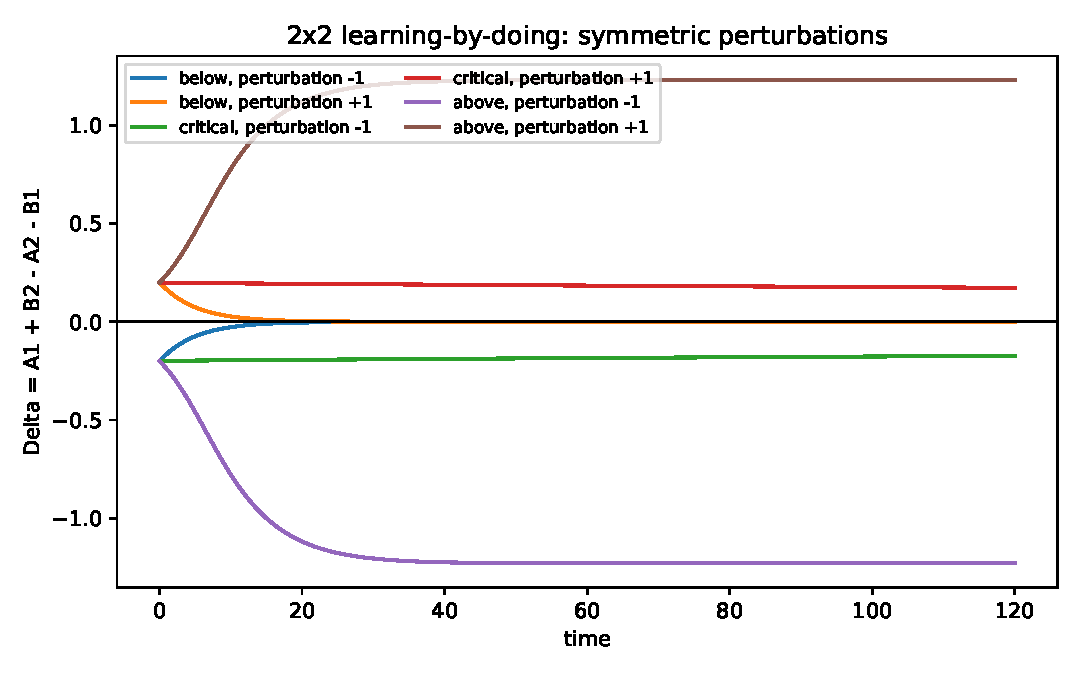
\includegraphics[width=0.82\linewidth]{../results/microverification/specialization_dynamics.pdf}
\caption{Diagnostic trajectories of the assignment gap in the symmetric learning-by-doing model. They verify the local-threshold calculation for one parameterisation; they are not empirical evidence of real HLS specialization.}
\label{fig:specialization}
\end{figure}

For CR1, $(\Delta_0,x,y)=(1,0.6,0.6)$ gives $G(x,0)=G(0,y)=0$ and $G(x,y)=0.2$. For CR4, an independent grid argmin matches Equation~\eqref{eq:rebalancing-solution} across TRAIN, boundary, MIXED, ROUTE, and selected limiting cases. The interior example $(d_0,a,v,g)=(1,1.5,1,1)$ yields $(x^*,y^*)=(0.5,0.5)$ and $Q_M=1.375<Q_T=Q_R=1.5$ (Figure~\ref{fig:rebalancing}).

\begin{figure}[t]
\centering
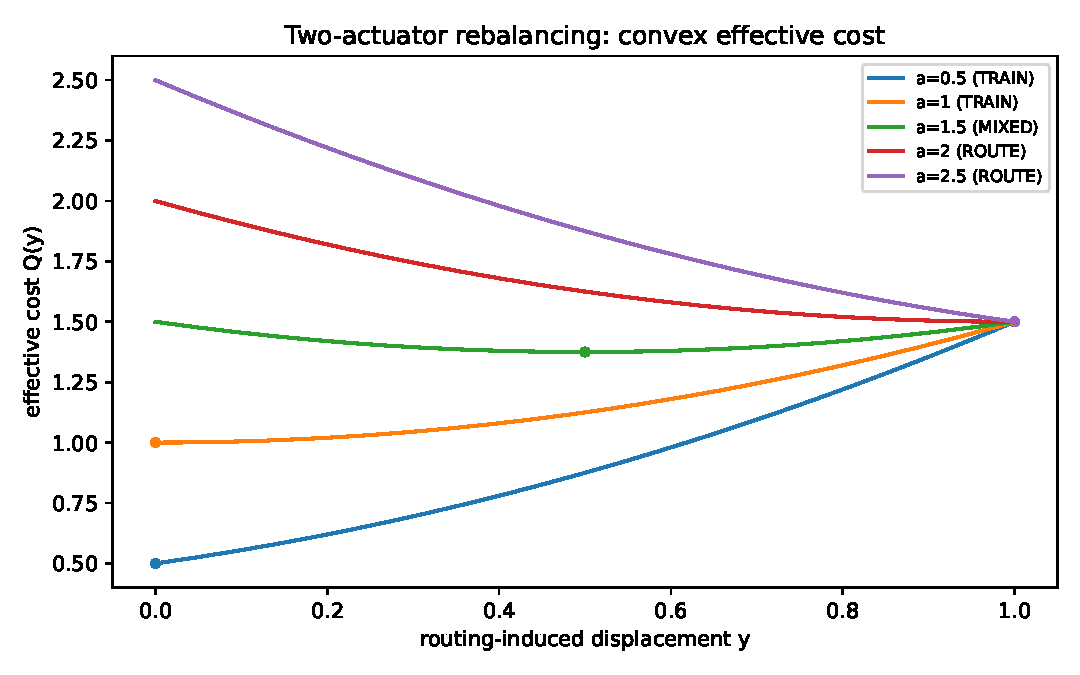
\includegraphics[width=0.82\linewidth]{../results/microverification/rebalancing_costs.pdf}
\caption{Diagnostic convex effective-cost curves for the two-actuator rebalancing calculation. The plotted parameter choices illustrate the closed-form TRAIN/MIXED/ROUTE regimes only.}
\label{fig:rebalancing}
\end{figure}

\section{Discussion and limitations}

\paragraph{Established in the model.} CR0 gives a separability null case. CR1 gives a threshold-based complementarity identity. CR2 gives a local instability threshold of the specified symmetric ODE. CR3--CR4 give deterministic scalar rebalancing identities.

\paragraph{Numerically verified.} The repository verifies the CR1 example, the symbolic and finite-difference Jacobian, the sign change of the local CR2 eigenvalue, selected perturbation trajectories, and the rebalancing formula against a grid argmin. Numerical agreement is a check of the implementation, not an independent empirical phenomenon.

\paragraph{Candidate architecture-level hypotheses.} It remains a hypothesis that real operational experience and direct learning can generate sufficiently different competence transformations to make deliberate competence evolution valuable. It remains a hypothesis that teacher buffering can support adaptation under persistent environmental change, and that specialization, broadening, replication, or rebalancing can improve future portfolio operation under realistic constraints.

\paragraph{Open novelty questions.} No novelty is claimed for the model, its mathematics, its components, or the paper framing. A later claim would require showing that substantially the same HLS phenomenon has not already been established for a genuinely equivalent learning-system class under comparable assumptions.

Strong adversaries include a sufficiently rich frozen heterogeneous portfolio with a strong adaptive router, free competence acquisition, complete future information and optimal ex-ante portfolio design, competence transitions independent of operation, and a fully informed modular controller. These are not peripheral caveats: they identify null cases in which deliberate competence evolution may add no value. In particular, neither the minimal mixed optimum nor local specialization establishes P4.

The minimal model omits uncertainty, demand drift, finite data, teachers, recipient heterogeneity, transfer, forgetting, interference, queues, latency constraints, and any demonstrated mapping from competence to real model accuracy. The general architecture names some of these roles but does not yet supply their transition laws, a final objective, an orchestration algorithm, or empirical evidence. These omissions preclude direct claims about deployed systems.

\section{Conclusion}

This working draft records a minimal dynamic language for asking how the distribution of usable competence in a heterogeneous portfolio might evolve through operation and learning. Within explicit toy assumptions, it establishes separability and threshold/control identities and verifies their implementation numerically. It does not establish a general HLS mechanism, a coupled-controller advantage, novelty, or practical value.

The central scientific objective remains whole-system HLS: knowledge or competence is the managed material; learning is the transformation mechanism; heterogeneity defines the portfolio; operation gives competence value; and time makes competence investment meaningful. Mathematical tools should serve that objective rather than define it.


\bibliographystyle{plainnat}
\bibliography{references}

\end{document}
